%
%  untitled
%
%  Created by Dean Freestone on 2010-07-06.
%  Copyright (c) 2010 . All rights reserved.
%
\documentclass[]{article}

% Use utf-8 encoding for foreign characters
\usepackage[utf8]{inputenc}

% Setup for fullpage use
\usepackage{fullpage}

% Uncomment some of the following if you use the features
%
% Running Headers and footers
%\usepackage{fancyhdr}

% Multipart figures
%\usepackage{subfigure}

% More symbols

%\usepackage{latexsym}

% Surround parts of graphics with box
\usepackage{boxedminipage}

% Package for including code in the document
\usepackage{listings}

% If you want to generate a toc for each chapter (use with book)
\usepackage{minitoc}

% This is now the recommended way for checking for PDFLaTeX:
\usepackage{ifpdf}

\usepackage{amsmath,amssymb,amsfonts,epsfig} % Typical maths resource packages

%\newif\ifpdf
%\ifx\pdfoutput\undefined
%\pdffalse % we are not running PDFLaTeX
%\else
%\pdfoutput=1 % we are running PDFLaTeX
%\pdftrue
%\fi

\ifpdf
\usepackage[pdftex]{graphicx}
\else
\usepackage{graphicx}
\fi
\usepackage{color}
\newcommand{\dean}[1]{\textsf{\emph{\textbf{\textcolor{red}{#1}}}}} 


\title{Patient-Specific Neural Field Modeling from Mirco-Electrode Data}
\author{In no specific order: Parham Aram, Dean R. Freestone, Kenneth Scerri, Michael Dewar,\\
 Jacob A. Donoghue, Sydney S. Cash, David B. Grayden and Visakan Kadirkamanathan  }

\date{2010-07-06}

\begin{document}

\ifpdf
\DeclareGraphicsExtensions{.pdf, .jpg, .tif}
\else
\DeclareGraphicsExtensions{.eps, .jpg}
\fi

\maketitle


\begin{abstract}
	
	\begin{itemize}
		\item Background
		\item Method
		\item Result
		\item Conclusion
	\end{itemize}
\end{abstract}

\section{Introduction}
\begin{itemize}
	\item Understanding of macroscopic neurodynamics
	\item Neural field model
	\item Improvements in electrode technology with great spatiotemporal resolution
\end{itemize}
The aim of this paper is to great a patient-specific neural field model, by estimating parameters of a general mathematical model using data acquired from an epilepsy surgical candidate in a clinical setting. 
\section{Method}

\subsection{Neural Field Model}
The neural field equations used as the parametric form of the model are based on the influential papers from Wilson and Cowan~\cite{Wilson1973}, and Amari~\cite{Amari1977}. This class of model describes a continuous cortical sheet or surface, relating mean firing rates of pre and post-synaptic neural populations. The neural field, $v\left( {\mathbf{r},t} \right)$, at position $\mathbf{r}$ and time $t$, is the aggregated post-synaptic potentials described by the temporal convolution 
\begin{equation}
	\label{SpikesToPotential} v\left( {\mathbf{r},t} \right) = \int_{ - \infty }^t {h\left( {t - t'} \right)g\left( {\mathbf{r},t'} \right)dt'}, 
\end{equation}   
where $h(\cdot)$ is the synaptic response kernel and $g(\cdot)$ describes the mean firing rate. Assuming an infinite propagation velocity for action potentials within the field, the incoming firing rate the position $\mathbf{r}$ is described by spatial convolution
\begin{equation}
	\label{RateBasedInteractions} g\left( \mathbf{r},t \right) = \int_\Omega {w\left( \mathbf{r},\mathbf{r}' \right)f\left( v\left( \mathbf{r}',t \right) \right)\textrm{d}\mathbf{r}'}, 
\end{equation}
where $w(\cdot)$ is the spatial connectivity kernel and $\Omega$ is the spatial domain representing the cortical sheet or surface. The function $f(\cdot)$ relates mean post-synaptic potentials to mean firing rates and follows a sigmoid described by
\begin{equation}
	\label{ActivationFunction} f\left( v\left( \mathbf{r}', t \right) \right) = \frac{1}{1 + \exp \left( \varsigma \left( v_0 - v\left(\mathbf{r}',t\right) \right) \right)}, 
\end{equation}
where $v_0$ and $\varsigma$ describe the firing threshold the slope of the sigmoid respectively. By substituting equation~\ref{RateBasedInteractions} into equation~\ref{SpikesToPotential} we get the spatiotemporal model 
\begin{equation}
	\label{FullDoubleIntModel} v\left(\mathbf{r},t\right) =
	\int_{-\infty}^t 
	h\left(t - t'\right) \int_\Omega
	w\left(\mathbf{r},\mathbf{r}'\right) 
	f\left( v\left( \mathbf{r}',t' \right)\right)
	\textrm{d}\mathbf{r}'dt'.
\end{equation}
To arrive at the general integral-differential equation form of the model, we shall express the synaptic response kernel as a Green's function 
\begin{equation}
	\label{GreensFuncDef} Dh\left( t \right) = \delta \left( t \right), 
\end{equation}
where $D$ is a temporal differential operator and $\delta(t)$ is the Dirac-delta function giving 
\begin{equation}
	\label{FinalFormContinuous} 
	Dv\left( \mathbf{r},t \right) = \int_\Omega {w\left( \mathbf{r},\mathbf{r}' \right)f\left( {v\left( \mathbf{r}',t \right)} \right)\textrm{d}\mathbf{r}'}. 
\end{equation}
By assuming the synaptic response kernel is of first order has the form of
\begin{equation}
	\label{SynapticRespKernel} h(t) = \eta(t)\exp{\left(-\zeta t\right)}, 
\end{equation}
where $\zeta=\tau^{-1}$, $\tau$ is the synaptic time constant and $\eta(t)$ is the Heaviside step function, the operator $D$ is
\begin{equation}
	D=\frac{d}{dt} + \zeta,
\end{equation}
yielding
\begin{equation}
	\label{FinalFormContinuous} 
	\frac{dv\left( \mathbf{r},t \right)}{dt} + \zeta v\left( \mathbf{r},t \right) = \int_\Omega {w\left( \mathbf{r},\mathbf{r}' \right)f\left( {v\left( \mathbf{r}',t \right)} \right)\textrm{d}\mathbf{r}'}. 
\end{equation}
The neural field equations must be written as a discrete-time finite-dimensional model in order to relate it to patient-specific data. The discrete-time model is found applying the a first-order Euler method giving
\begin{equation}\label{EulerMethod}
	\frac{v\left( \mathbf{r},t+T_s \right)-v\left( \mathbf{r},t \right)}{T_s} + \zeta v\left(\mathbf{r},t \right) = \int_\Omega {w\left( \mathbf{r},\mathbf{r}' \right) f\left( {v\left( \mathbf{r}',t \right)}\right)\textrm{d}\mathbf{r}'},
\end{equation}
where $T_s$ is the time step or sampling period. To simplify the notation, the sample at the the current time step shall be indexed by $t$ and the future time step by $t+1$ for the rest of the paper. Rearranging equation~\ref{EulerMethod} gives the integro-difference equation (IDE) form
\begin{equation}
	\label{DiscreteTimeModel} 
	v_{t+1}\left(\mathbf{r}\right) = 
	\xi v_t\left(\mathbf{r}\right) + 
	T_s \int_\Omega { 
	    w\left(\mathbf{r},\mathbf{r}'\right)
	    f\left(v_t\left(\mathbf{r}'\right)\right) 
	\textrm{d}\mathbf{r}'}, 
\end{equation}
where $\xi = 1-T_s\zeta$. Finally, a disturbance term is added, to account for uncertainty and unmodelled inputs, to the IDE form giving
\begin{equation}
	\label{NoisyDiscreteTimeModel} 
	v_{t+1}\left(\mathbf{r}\right) = 
	\xi v_t\left(\mathbf{r}\right) + 
	T_s \int_\Omega { 
	    w\left(\mathbf{r},\mathbf{r}'\right)
	    f\left(v_t\left(\mathbf{r}'\right)\right) 
	\textrm{d}\mathbf{r}'} 
	+ e_t\left(\mathbf{r}\right), 
\end{equation}
where $e_t(\mathbf{r})$ is $i.i.d.$ such that $e_t(\mathbf{r})\sim\mathcal{GP}(\mathbf 0,\gamma(\mathbf{r}-\mathbf{r}'))$. Here $\mathcal{GP}(\mathbf 0,\gamma(\mathbf{r}-\mathbf{r}'))$ denotes a zero mean spatial Gaussian process with covariance function $\gamma(\mathbf{r}-\mathbf{r}')$~\cite{Rasmussen2005}.
To reduce the model to a finite-dimensional system the neural field is approximated by a basis function decomposition where
\begin{equation}
	\label{DefFieldDecomp} v_t\left(\mathbf{r}\right) \approx \boldsymbol{\phi}^{\top}\left(\mathbf{r}\right) \mathbf{x}_t 
\end{equation}
and $\mathbf{x}_t$ is a state vector that weights a vector of two-dimension Gaussian basis functions, $\boldsymbol{\phi}(\mathbf{r})$, described by
\begin{equation}\label{eq:FieldBasisFunction}
	\boldsymbol\phi\left(\mathbf{r}-\mathbf{r}'\right) =
\exp{\left(-\frac{(\mathbf{r}-\mathbf{r}')^\top(\mathbf{r}-\mathbf{r}')}{\sigma_{\phi}^2}\right)}. 
\end{equation}
The parameter $\sigma_{\phi}$ controls the basis function width and is inferred by frequency analysis. Substituting equation~\ref{DefFieldDecomp} into~\ref{NoisyDiscreteTimeModel} gives to approximate model
\begin{equation}
	\label{eq:reduced continuous model}
	\boldsymbol{\phi}^{\top}(\mathbf{r})\mathbf{x}_{t+1}= T_s\int_\Omega{f(\boldsymbol{\phi}^{\top}(\mathbf{r}')\mathbf{x}_t )w(\mathbf{r},\mathbf{r}')\textrm{d}\mathbf{r}'}
	+ \xi\boldsymbol{\phi}^{\top}(\mathbf{r})x_t + e_t(\mathbf{r}). 
\end{equation}
Next we multiply equation~\ref{eq:reduced continuous model} by $\boldsymbol{\phi}(\mathbf{r})$ and integrate over the spatial domain, $\Omega$, to get 
\begin{equation}
	\label{StartofReduction}
 	\int_\Omega {\boldsymbol{\phi} \left(\mathbf{r}\right)\boldsymbol{\phi}^{\top}\left(\mathbf{r}\right) \textrm{d}\mathbf{r}} \mathbf{x}_{t+1} = T_s \int_\Omega {\boldsymbol{\phi} (\mathbf{r}) \int_\Omega {w(\mathbf{r},\mathbf{r}') f(\boldsymbol{\phi}^{\top}(\mathbf{r}') \mathbf{x}_t ) \textrm{d}\mathbf{r}'}\textrm{d}\mathbf{r}} + \xi\int_\Omega{\boldsymbol{\phi}(\mathbf{r})\boldsymbol{\phi}^{\top}(\mathbf{r})\textrm{d}\mathbf{r}} \mathbf{x}_t + \int_\Omega{\boldsymbol{\phi} (\mathbf{r}) e_t(\mathbf{r})\textrm{d}\mathbf{r}}. 
\end{equation}
Now by defining the matrix
\begin{equation}\label{eq:DefGamma}
	\boldsymbol{\Gamma} \triangleq \int_\Omega {\boldsymbol{\phi} \left(\mathbf{r}\right)\boldsymbol{\phi} ^{\top}\left(\mathbf{r}\right)\textrm{d}\mathbf{r}} 
\end{equation}
enables the pseudo inverse of $\boldsymbol{\phi(\mathbf{r})}$ to be taken, such that the state vector can is isolated on the left-hand-side as
\begin{equation}\label{eq:ReducedForm}
	 \mathbf{x}_{t+1} = T_s\boldsymbol{\Gamma}^{-1}
	 \int_\Omega \boldsymbol{\phi}(\mathbf{r}) 
	 \int_\Omega w(\mathbf{r},\mathbf{r}')f(\boldsymbol{\phi}^{\top}(\mathbf{r}')\mathbf{x}_t) \textrm{d}\mathbf{r}' \textrm{d}\mathbf{r} 
	 + \xi\mathbf{x}_t + \boldsymbol{\Gamma}^{-1} \int_\Omega{\boldsymbol{\phi}(\mathbf{r}) e_t(\mathbf{r})\textrm{d}\mathbf{r}}.
\end{equation}
A property of the Gaussian basis function decomposition it that the Gaussianality of the disturbance term is maintained. The decomposition disturbance term is defined as
\begin{equation}\label{eq:Wt} 
	\mathbf{e}_t \triangleq \boldsymbol{\Gamma}^{-1}\int_\Omega {\boldsymbol{\phi} ( \mathbf{r} )e_t( \mathbf{r} )\textrm{d}\mathbf{r}},
\end{equation}
where $\mathbf{e}_t \sim\mathcal{N}(\mathbf 0,\boldsymbol\Sigma_e)$. The covariance matrix is defined as (see the Supporting Information, S1, for the derivation)
\begin{equation}
	\boldsymbol\Sigma_e \triangleq \mathbf{\Gamma}^{-1}\int_{\Omega}\int_{\Omega}\boldsymbol{\phi}\left(\mathbf r\right) \gamma\left(\mathbf r- \mathbf r' \right)\boldsymbol{\phi}\left(\mathbf r'\right)^{\top}d\mathbf r' d\mathbf r\mathbf{\Gamma}^{- \top}. 
\end{equation}

\subsection{Data Collection and Pre-processing}

Data was collected from a patient undergoing work-up for surgical resection of epileptic brain tissue. The standard procedure for the resective surgery involves implantation of subdural electrodes for intracranial EEG monitoring (iEEG). Data from these electrodes provide information for mapping functional and pathological tissue to define the surgical margins. In addition to standard iEEG electrodes, data was collected in parallel from a Neuroport system (Blackrock microsystems, Utah, USA) incorporating a micro-electrode array. This data was collected with informed consent from the patient under ethics approval from the MGH human research ethics committee..?? Figure~\ref{MRI_CT} shows the position of the iEEGs electrodes and the micro-electrode array. The iEEG electrode covers the temporal lobe, and the micro-electrode placement was targeted at.. The micro-electrode array consisted of square grid of 96 (10 by 10 with the corner electrodes missing). The x,y electrode spacing was 400~$\mu m$, yielding a coverage of 4 by 4~mm. Data from the Neuroport system was acquired with a sampling rate of 30~kHz, with hardware filters in the range of~\dean{??}. 

During the time-course of the iEEG monitoring several seizures were recorded. This study focuses on the local field potential (LFP) data recorded with the micro-electrode during a seizure. 

The first pre-processing step was to identify channels that had very poor signal quality. These channels were set to the $nan$ data type. Following this, the data was re-referenced to a common average montage to remove common mode artifact and the effect of the reference electrode. Next the data was low-pass filtered with a cut-off frequency of 100~Hz. The data was then resampled from 30~kHz to 5~kHz. To enable spatial visualisation and spatial frequency analysis, the corrupted channels, set to $nan$, were interpolated using all neighbouring channels.

\subsection{Spatiotemporal Data Analysis}
The first 8 channels of the LFP time series from the seizure is shown in Figure~\ref{fig:TimeSeries}. For the analysis, the time series was segmented into three periods; the pre-seizure period, seizure period and post-seizure period. The seizure onset is marked by the red dotted line and the seizure end is marked by the blue dashed line. 

\begin{figure}[!ht]
\begin{center}
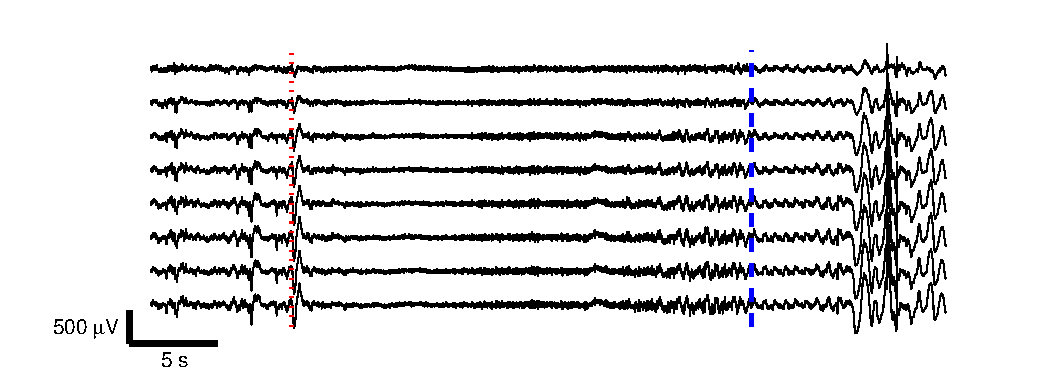
\includegraphics{./Figures/LFPs.eps}
\end{center}
\caption{{\bf Local field potentials from the micro-electrode array}. Data recorded from the first 8 channels of the array. The red dotted line indicates the seizure onset and the blue dashed line indicates the seizure end.}
\label{fig:TimeSeries}
\end{figure}

An example to illustrate the spatial aspects of the observed neural field is shown in Figure~\ref{fig:FieldObserations}. Each subplot in the figure shows the observed field at a sample of the pre-processed data, with each plot separated in time by 2.5~ms. The figure shows spatially correlated activity.

\begin{figure}[!ht]
\begin{center}
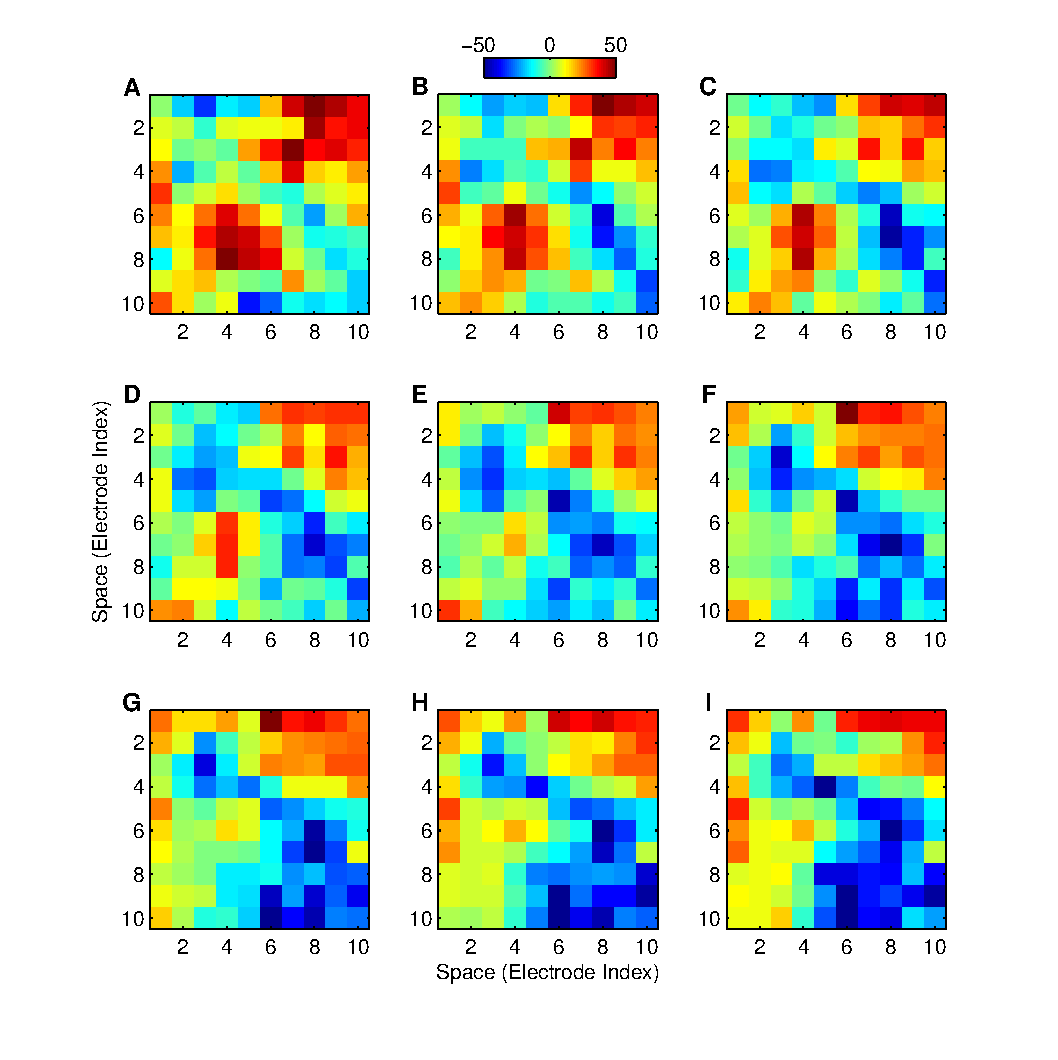
\includegraphics{./Figures/FieldObservations.eps}
\end{center}
\caption{{\bf Snap-shots of the spatial aspects of the observed field}. The snap-shots are ordered from A to I forming a consecutive sequence spaced 2.5~ms apart starting at 34.024s}
\label{fig:FieldObserations}
\end{figure}

The spectral properties of the recorded time series for each of the time segments are shown in Figure~\ref{fig:TemporalFreqObservation}. Each plot shows an averaged (across channels) spectrum the data. The pre-seizure period shows a decay in power at a typical $1/f^2$ rate. The seizure period has higher power at low and high ends of the spectrum. In addition, there is a peak in the power of the LFPs at ~51~Hz during the seizure. This peak would be difficult to observe in European and Asian countries due to the 50~Hz mains power frequency. The post-seizure period shows a large increase in lower frequency power...
 
\begin{figure}[!ht]
\begin{center}
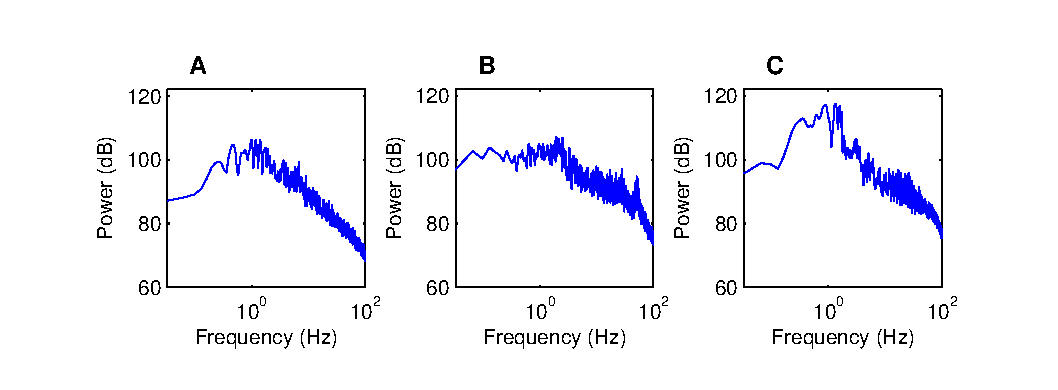
\includegraphics{./Figures/TemporalFreq.eps}
\end{center}
\caption{{\bf Spectra from local field potential recordings}. A. Pre-seizure observations. B. Seizure observations. C. Post-seizure observations.}
\label{fig:TemporalFreqObservation}
\end{figure}

Figure~\ref{fig:SpatialFreqObservation} shows the results of spatial frequency analysis of the observed neural field. Throughout this paper the spatial frequency shall be denoted by $\nu$. Each subplot is an average (across time) spatial frequency during either the pre-seizure, seizure or post-seizure periods. The spatial frequency of the neural field is governed by disturbances (inputs from outside the field) and the underlying connectivity structure. The symmetry in the plots provides some evidence for homogeneous and isotropic connectivity.   

\begin{figure}[!ht]
\begin{center}
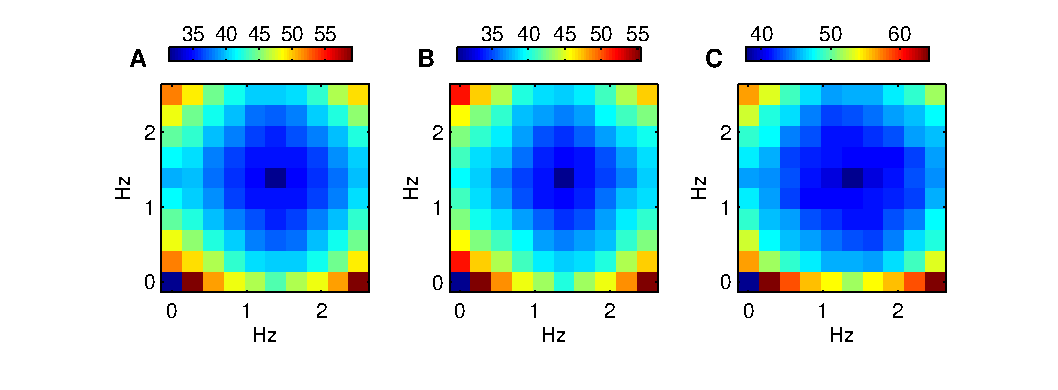
\includegraphics{./Figures/SpatialFreq.eps}
\end{center}
\caption{{\bf Spatial frequency analysis of the observed neural field}. A. Pre-seizure observations. B. Seizure observations. C. Post-seizure observations.}
\label{fig:SpatialFreqObservation}
\end{figure}

Figure~\ref{fig:DiagSpatialFreqObservation} shows diagonal cross-sections of the spatial frequency plots. From this figure we can see that the spatial cut-off frequency (-3~dB point) is $\nu_c \approx 0.26$~Hz. The profile of the diagonal cross-section indicates that the field is adequately sampled from the micro-electrode array, where the power drops by ~25~dB at the maximum observable spatial frequency (according to Shannon's sampling theorem) indicating spatial aliasing will have an insignificant effect. The spatial cut-off frequency provides information on the complexity of the model required to represent the neural field. Considering the field is band-limited, we can represent the continuous field by a finite set of continuous basis functions. According the Shannon's sampling theorem, the minimum spacing between basis functions, $\Delta_{\phi}$, to describe the field is
\begin{equation}\label{eq:BasisFunctionSeparation}
	\Delta_{\phi} \leq \frac{1}{2\rho_{\phi}\boldsymbol{\nu}_{c}}
\end{equation}
where $\rho_{\phi} \in \mathbb{R} \ge 1$ is an oversampling parameter to determine the basis function separation.



\begin{figure}[!ht]
\begin{center}
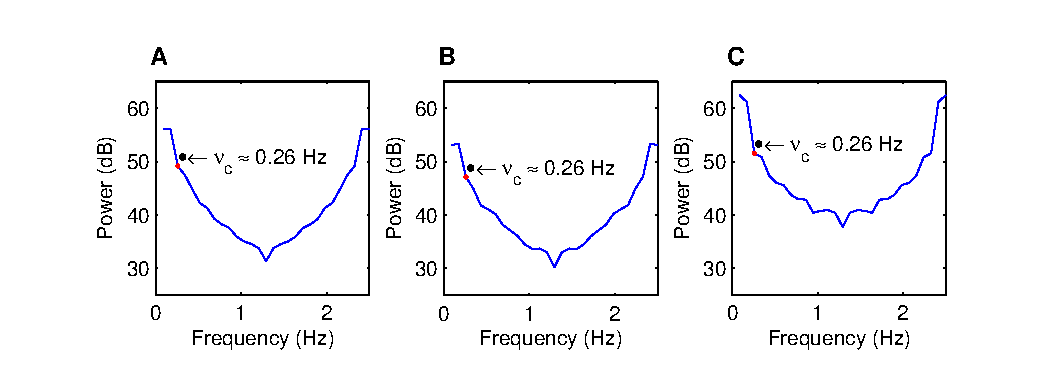
\includegraphics{./Figures/SpatialFreqCrossSection.eps}
\end{center}
\caption{{\bf Diagonal cross-section of the spatial frequency plots of the observed neural field}. A. Pre-seizure observations. B. Seizure observations. C. Post-seizure observations.}
\label{fig:DiagSpatialFreqObservation}
\end{figure}

\subsection{Estimating Support For Connectivity Kernel}
The support for the connectivity kernel can be inferred...

\begin{figure}[!ht]
\begin{center}
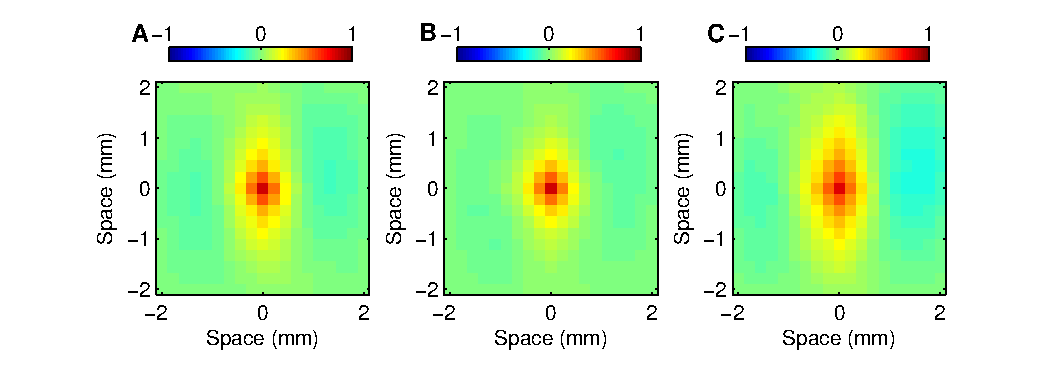
\includegraphics{./Figures/CrossCorr2D.eps}
\end{center}
\caption{{\bf Mean cross-correlations between consecutive observations of the neural field}. Note: The correlations are normalised such that the maximum value is one. A. Pre-seizure observation correlations. B. Seizure observation correlations. C. Post-seizure observation correlations.}
\label{fig:SpatialCrossCorrelation}
\end{figure}

\begin{figure}[!ht]
\begin{center}
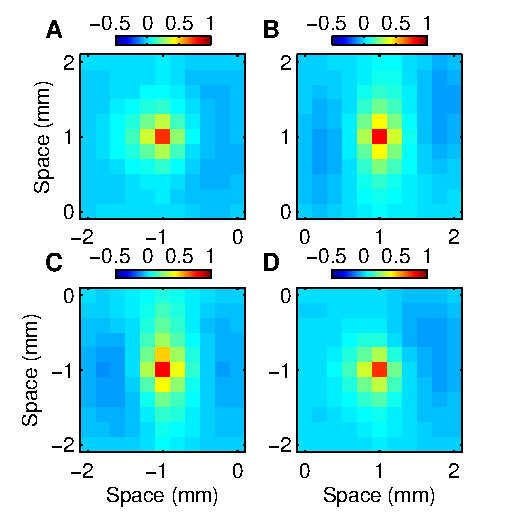
\includegraphics{./Figures/HomoTestCrossCorr.eps}
\end{center}
\caption{{\bf Mean cross-correlations between consecutive samples using subsets of observations of the neural field}. Each subplot shows correlations corresponding to a subset electrodes. Indexing the electrodes in a (x,y) grid, where index ranges from 1 to 10. Subplot A shows the mean correlation between electrode indexes (1-6, 5-10), subplot B shows correlations from indexes (5-10,5-10), subplot C shows indexes (1-6, 1-6) and subplot D shows indexes (5-10, 5-10).}
\label{fig:HomogeneityTest}
\end{figure}


\subsection{Estimation Algorithm}
The state space model is given by
\begin{equation}
 \mathbf x_{t+1}=\boldsymbol\Theta q(\mathbf x_t)+\xi \mathbf x_t+\boldsymbol e_t(\mathbf r)
\end{equation}
\begin{equation}
 \mathbf y_t=\mathbf C \mathbf x_t+\boldsymbol \epsilon_t
\end{equation}
where $\boldsymbol\Theta$ is an $n_x \times n_x$ block matrix where each block matrix is of dimension $ 1\times n_{\theta}$ defined as
\begin{equation}
\boldsymbol \Theta_{i,j}=\left\lbrace  \begin{array}{cc}
\boldsymbol \theta^\top &i=j \\
\mathbf 0_{1 \times n_{\theta}}& i\neq j  
 \end{array}\right. 
\end{equation}
and the non-linear map $q(.)$ is defined as
\begin{equation}\label{eq:QmatrixForSigmapoints}
	q(\mathbf{x}_t) \triangleq T_s\boldsymbol{\Gamma}^{-1} \int_\Omega \boldsymbol{\Lambda}(\mathbf{r}') f(\boldsymbol{\phi}^{\top}(\mathbf{r}')\mathbf{x}_t) d\mathbf{r}'.
\end{equation}
where $\boldsymbol{\Lambda}(\mathbf{r}')  $ is an $n_x \times 1$ block vector with each block of dimension $n_{\theta} \times 1 $
\begin{equation}\label{eq:DefPsi}
\boldsymbol{\Lambda}(\mathbf{r}')=\begin{bmatrix}\boldsymbol \lambda_1(\mathbf r')\\\boldsymbol \lambda_2(\mathbf r')\\ \vdots \\ \boldsymbol \lambda_{n_{x}}(\mathbf r') \end{bmatrix}_{n_x \times 1}
\end{equation}
and where
\begin{equation}
\boldsymbol \lambda_i(\mathbf r') =\begin{bmatrix} \phi_i\ast \psi_1(\mathbf r') \\ \phi_i\ast \psi_2 (\mathbf r') \\ \vdots \\ \phi_i\ast \psi_{n_{\theta}}(\mathbf r') \end{bmatrix}_{n_{\theta} \times 1}
\end{equation}
As a result $q(\mathbf x_t)$ is an $n_x \times 1$ block vector and each block is $n_{\theta} \times 1$. It should be noted that $\boldsymbol\Theta q(\mathbf x_t)$ is an $n_x \times 1$ vector.
$ \boldsymbol e_t(\mathbf r)\sim \mathcal N(\mathbf 0,\boldsymbol\Sigma_e(\mathbf r,\mathbf r'))$ is temporally white and spatially colored disturbance and  $\boldsymbol\epsilon_t\sim \mathcal N(\mathbf 0,\boldsymbol\Sigma_{\epsilon})$ is a white noise process.
\subsection*{$\mathcal Q$-function}
Expanding the joint distribution $p(\mathbf X,\mathbf Y;\boldsymbol \theta,\xi)$ we have
\begin{equation}
 p(\mathbf X,\mathbf Y;\boldsymbol \theta,\xi)=\prod_{t=1}^{T} p(\mathbf y_t|\mathbf x_t)p(\mathbf x_t|\mathbf x_{t-1};\boldsymbol \theta, \xi)p(\mathbf x_0)
\label{eq:jointdistribution}
\end{equation}
The $\mathcal Q$-function can be written in terms of its component as shown in (\ref{eq:jointdistribution})
\begin{eqnarray}
 \mathcal Q(\boldsymbol \theta,\xi,\boldsymbol\theta',\xi')&=&\mathbf E_{\boldsymbol (\theta',\xi')}[\ln p(\mathbf X,\mathbf Y;\boldsymbol \theta,\xi)]\nonumber\\
&=&\mathbf E_{\boldsymbol (\theta',\xi')}[\sum_{t=1}^{T}\ln p(\mathbf y_t|\mathbf x_t)+\sum_{t=1}^{T}\ln p(\mathbf x_t|\mathbf x_{t-1};\boldsymbol \theta)+\sum_{t=1}^{T}\ln p(\mathbf x_0)]
\end{eqnarray}
$p(\mathbf y_t|\mathbf x_t)$ and $p(\mathbf x_0)$ are not functions of parameter therefore $\mathcal Q$-function can be rewritten as
\begin{equation}
\mathcal Q(\boldsymbol \theta,\xi,\boldsymbol\theta',\xi')=\mathbf E_{(\theta',\xi')}[\sum_{t=1}^{T}\ln p(\mathbf x_t|\mathbf x_{t-1};\boldsymbol \theta ,\xi)]+\textrm{const}
\end{equation}
The Gaussian distribution of the disturbance, $e_t(\mathbf r)\sim \mathcal N(\mathbf 0,\boldsymbol\Sigma_e(\mathbf r,\mathbf r'))$ results into the following conditional distribution of the state at $t+1$
\begin{equation}
 p(\mathbf x_{t+1} | \mathbf x_t;\boldsymbol\theta,\xi)=ce^{-(\mathbf x_{t+1}-\boldsymbol\Theta q(\mathbf  x_t)-\xi  \mathbf x_t)^\top\boldsymbol\Sigma_e^{-1}(\mathbf x_{t+1}-\boldsymbol\Theta q( \mathbf x_t)-\xi \mathbf  x_t)}
\end{equation}
where c is the normalising constant. Taking $\log$ we get
\begin{equation}
 \ln p(\mathbf x_{t+1} |\mathbf x_t;\boldsymbol\theta,\xi)=\ln c -(\mathbf x_{t+1}^\top-q^\top(\mathbf x_t)\boldsymbol\Theta^\top -\xi  \mathbf x_t^\top)\boldsymbol\Sigma_e^{-1}(\mathbf x_{t+1}-\boldsymbol\Theta q(\mathbf x_t)-\xi \mathbf x_t)
\end{equation}
\begin{eqnarray}
 \ln p(\mathbf x_{t+1} | \mathbf x_t;\boldsymbol\theta, \xi)&=&\ln c-[\mathbf x_{t+1}^\top\boldsymbol\Sigma_e^{-1}\mathbf x_{t+1}-\mathbf x_{t+1}^\top\boldsymbol\Sigma_e^{-1}\boldsymbol\Theta q(\mathbf x_t)-\xi \mathbf x_{t+1}^\top\boldsymbol\Sigma_e^{-1}\mathbf x_t \nonumber \\
&&- q^\top(\mathbf x_t)\boldsymbol\Theta^\top\boldsymbol\Sigma_e^{-1}\mathbf x_{t+1}+q^\top(\mathbf x_t)\boldsymbol\Theta^\top\boldsymbol\Sigma_e^{-1}\boldsymbol\Theta q(\mathbf x_t)+\xi q^\top(\mathbf x_t)\boldsymbol\Theta^\top \boldsymbol\Sigma_e^{-1}\mathbf x_t \nonumber\\
&&-\xi \mathbf x_t^\top\boldsymbol\Sigma_e^{-1}\mathbf x_{t+1}+\xi  \mathbf  x_t^\top\boldsymbol\Sigma_e^{-1}\boldsymbol\Theta q(\mathbf x_t)+\xi^2\mathbf x_t^\top\boldsymbol\Sigma_e^{-1}\mathbf x_t]
\end{eqnarray}
\begin{eqnarray}\label{eq:Qfunctioninter}
  \ln p(\mathbf x_{t+1} | \mathbf x_t;\boldsymbol\theta,\xi)&=&\ln c-\mathbf x_{t+1}^\top\boldsymbol\Sigma_e^{-1}\mathbf x_{t+1}+2\mathbf x_{t+1}^\top\boldsymbol\Sigma_e^{-1}\boldsymbol\Theta q( \mathbf x_t)+2\xi \mathbf x_{t+1}^\top\boldsymbol\Sigma_e^{-1}\mathbf x_t\nonumber \\
&&-q^\top(\mathbf x_t)\boldsymbol\Theta^\top \boldsymbol\Sigma_e^{-1}\boldsymbol\Theta q(\mathbf x_t)-2\xi \mathbf x_t^\top\boldsymbol\Sigma_e^{-1}\boldsymbol\Theta q(\mathbf x_t)-\xi^2\mathbf x_t^\top\boldsymbol\Sigma_e^{-1}\mathbf x_t
\end{eqnarray}
taking trace and using invariant cyclic permutations property of the trace this distribution can be written as 
 \begin{eqnarray}
   \ln p(x_{t+1} | \mathbf x_t;\boldsymbol\theta,\xi)&=&\ln c-\mathbf x_{t+1}^\top\boldsymbol\Sigma_e^{-1}\mathbf x_{t+1}+2 tr \left\lbrace  \boldsymbol\Theta q( \mathbf x_t)\mathbf x_{t+1}^\top\boldsymbol\Sigma_e^{-1}\right\rbrace  +2 \xi tr\left\lbrace \mathbf x_t\mathbf x_{t+1}^\top\boldsymbol\Sigma_e^{-1}\right\rbrace  \nonumber\\
 &&-tr \left\lbrace \boldsymbol\Theta q(\mathbf x_t)q^\top(\mathbf x_t)\boldsymbol\Theta^\top \boldsymbol\Sigma_e^{-1}\right\rbrace  -2\xi tr \left\lbrace \boldsymbol\Theta q(\mathbf x_t)  \mathbf x_t^\top\boldsymbol\Sigma_e^{-1} \right\rbrace -\xi^2 tr \left\lbrace\mathbf x_t\mathbf x_t^\top\boldsymbol\Sigma_w^{-1} \right\rbrace  \nonumber
 \end{eqnarray} 
taking the expected value is leading to the following  $\mathcal Q$-function
\begin{eqnarray}
 \mathcal Q(\boldsymbol \theta,\xi,\boldsymbol\theta',\xi')&=&\beta+2 tr\left\lbrace \boldsymbol\Theta\Xi_2\boldsymbol\Sigma_e^{-1}\right\rbrace +2\xi tr \left\lbrace  \Xi_0\boldsymbol\Sigma_e^{-1}\right\rbrace  \nonumber \\
&-&tr \left\lbrace\boldsymbol\Theta\Xi_4 \boldsymbol\Theta^\top\boldsymbol\Sigma_e^{-1}\right\rbrace -2\xi tr \left\lbrace \boldsymbol\Theta\Xi_3\boldsymbol\Sigma_e^{-1}\right\rbrace  \nonumber \\
&-&\xi^2 tr \left\lbrace \Xi_1\boldsymbol\Sigma_e^{-1}\right\rbrace  \nonumber
\end{eqnarray}
where  $\beta= \sum_{t=1}^T\mathbf E_{(\theta',\xi)}[ \ln c-\mathbf x_{t+1}^\top\boldsymbol\Sigma_w^{-1}\mathbf x_{t+1}]$ is constant with respect to the parameters and will disapear by differentiation and 
\begin{equation}
 \Xi_0=\sum_{t=1}^T\mathbf E_{(\theta',\xi')}[\mathbf x_t\mathbf x_{t+1}^\top] \quad \Xi_1=\sum_{t=1}^T\mathbf E_{(\theta',\xi')}[\mathbf x_t\mathbf x_t^\top]
\end{equation}
Other terms can be approximated by linearising $q(\mathbf x)$ and taking the first-order truncated  Taylor-series expansion around the mean of the state at each time instant, i.e. 
\begin{equation}\label{eq:qTaylor}
 q(\mathbf x_t)\approx q(\hat{\mathbf x}_t)+\nabla^\top q (\hat{\mathbf x}_t)(\mathbf x_t -\hat{\mathbf x}_t)
\end{equation}
where
\begin{equation}
\nabla q=\begin{bmatrix}\frac{\delta q}{\delta x_{t,1}} \mid_{{\mathbf x}_t=\mathbf{\hat x}_t} &\frac{\delta q}{\delta x_{t,2}} \mid_{{\mathbf x}_t=\mathbf{\hat x}_t}& \dots &\frac{\delta q}{\delta x_{t,n}} \mid_{{\mathbf x}_t=\mathbf{\hat x}_t}\end{bmatrix}^\top
\end{equation}
and
\begin{equation}
\frac{\delta q}{\delta x_{t,i}}= \int_\Omega \boldsymbol{\Psi}(\mathbf{r}')\phi_i(\mathbf r') f'(\phi^\top(\mathbf{r}'){x}_t) d\mathbf{r}'\\
\end{equation}

therefore
\begin{equation}
 \Xi_2=\sum_{t=1}^{T}\mathbf E_{(\theta',\xi')}[q(\mathbf x_t)\mathbf x_{t+1}^\top ], \quad \mathbf E_{(\theta',\xi')}[q(\mathbf x_t)\mathbf x_{t+1}^\top ]\approx q(\mathbf{ \hat x}_t)\mathbf{ \hat x}_{t+1}^\top+\nabla^\top q(\mathbf{ \hat x}_t)\mathbf M_t
\end{equation}
\begin{equation}
 \Xi_3=\sum_{t=1}^{T}\mathbf E_{(\theta',\xi')}[q(\mathbf x_t)\mathbf x_{t}^\top ], \quad \mathbf E_{(\theta',\xi')}[q(\mathbf x_t)\mathbf x_{t}^\top ]\approx q(\mathbf{ \hat x}_t)\mathbf{ \hat x}_{t}^\top+\nabla^\top q(\mathbf{ \hat x}_t)\mathbf P_t
\end{equation}
\begin{equation}
 \Xi_4=\sum_{t=1}^{T}\mathbf E_{(\theta',\xi')}[q(\mathbf x_t)q^\top(\mathbf x_t) ], \quad \mathbf E_{(\theta',\xi')}[q(\mathbf x_t)q^\top(\mathbf x_t) ] \approx q(\mathbf{ \hat x}_t)q^\top(\mathbf{ \hat x}_t)+\nabla^\top q(\mathbf{ \hat x}_t)\mathbf P_t\nabla q(\mathbf{ \hat x}_t)
\end{equation}
we rewrite the $\mathcal Q$-function as
\begin{eqnarray}\label{eq:rewrittenQ}
 \mathcal Q(\boldsymbol \theta,\xi,\boldsymbol\theta',\xi')&=&\beta+2  \sum_{i,j,k=1}^{n_x}[\boldsymbol\Theta]_{i,j}[\Xi_2]_{j,k}[\boldsymbol\Sigma_e^{-1}]_{k,i} +2\xi tr \left\lbrace  \Xi_0\boldsymbol\Sigma_e^{-1}\right\rbrace  \nonumber \\
&-& \sum_{i,j,k,l=1}^{n_x}[\boldsymbol\Theta]_{i,j}[\Xi_4]_{j,k}[ \boldsymbol\Theta^\top]_{k,l}[\boldsymbol\Sigma_e^{-1}]_{l,i} -2\xi \sum_{i,j,k=1}^{n_x}[\boldsymbol\Theta]_{i,j}[\Xi_3]_{j,k}[\boldsymbol\Sigma_e^{-1}]_{k,i}  \nonumber \\
&-&\xi^2 tr \left\lbrace \Xi_1\boldsymbol\Sigma_e^{-1}\right\rbrace  
\end{eqnarray}
we can simplify \eqref{eq:rewrittenQ} by noting that $[\boldsymbol \Theta]_{i,j}=\mathbf 0 \quad i \neq j$ 

\begin{equation}
 \mathcal Q(\boldsymbol \theta,\xi,\boldsymbol\theta',\xi')=\beta +2\xi r_0 -\xi^2 r_1 +2 \boldsymbol\theta^\top \mathbf r_2-2\xi \boldsymbol\theta^\top \mathbf r_3  -\boldsymbol\theta^\top\mathbf R_4\boldsymbol\theta 
\end{equation}
where 
\begin{equation}
 r_0=tr \left\lbrace  \Xi_0\boldsymbol\Sigma_e^{-1}\right\rbrace   \quad r_1=tr \left\lbrace \Xi_1\boldsymbol\Sigma_e^{-1}\right\rbrace \quad
 \mathbf r_2=tr\left\lbrace \Xi_2\boldsymbol\Sigma_e^{-1}\right\rbrace \quad  \mathbf r_3= tr \left\lbrace \Xi_3\boldsymbol\Sigma_e^{-1}\right\rbrace \quad \mathbf R_4= tr \left\lbrace\Xi_4 \boldsymbol\Sigma_e^{-1}\right\rbrace\nonumber 
\end{equation}

differentiate with respect to $\boldsymbol\theta$ and equating to zero we have
\begin{eqnarray}
\frac{\delta \mathcal Q}{\delta \boldsymbol \theta}=2\mathbf r_2^\top-2\xi \mathbf r_3^\top-2\boldsymbol \theta^\top\mathbf R_4^\top=0
\end{eqnarray}
therefore
\begin{equation}\label{eq:thetasolution}
 \boldsymbol \theta=\mathbf R_4^{-1}(\mathbf r_2-\xi\mathbf r_3)
\end{equation}
differentiate with respect to $\xi$ we have
\begin{equation}
 \frac{\delta \mathcal Q}{\delta \xi}=+2r_0-2\xi r_1-2\boldsymbol\theta^\top\mathbf r_3=0
\end{equation}
and we get
\begin{equation}\label{eq:xisolution}
 \xi=\frac{1}{r_1}(r_0- \boldsymbol \theta^\top \mathbf r_3)
\end{equation}
substituting \eqref{eq:thetasolution} in \eqref{eq:xisolution} we get
\begin{eqnarray}
\xi=\frac{r_0-r'_0}{r_1-r'_1}
\end{eqnarray}
where
\begin{equation}
 r'_0=\mathbf r_2^\top \mathbf R_4^{-\top}\mathbf r_3 \quad r'_1=\mathbf r_3^\top \mathbf R_4^{-\top}\mathbf r_3
\end{equation}
and subsequently
\begin{equation}
 \boldsymbol \theta=\mathbf R_4^{-1}(\mathbf r_2+\frac{r'_0-r_0}{r_1-r'_1} \mathbf r_3)
\end{equation}
\subsection*{Discussion}
The second derivative of the $\mathcal Q$-function with respect to $\xi$ is given by
\begin{equation}
 \frac{\delta^2 \mathcal Q}{\delta \xi^2}=-2 r_1 \quad r_1=tr \left\lbrace \Xi_1\boldsymbol\Sigma_e^{-1}\right\rbrace
\end{equation}
$\Xi_1 $ is positive definite if the state vector is persistently excited and the covariance matrix $\boldsymbol\Sigma_w^{-1}$ is also positive definite therefore the trace of $\Xi_1\boldsymbol\Sigma_w^{-1}$ is guaranteed to be positive so the second derivative is negative and represents a maximum of $\mathcal Q$-function.\\
The second derivative of the $\mathcal Q$-function with respect to $\boldsymbol \theta$ is given by
\begin{equation}
 \frac{\delta^2 \mathcal Q}{\delta \boldsymbol\theta^2}=-2\mathbf R_4 \quad \mathbf R_4= tr \left\lbrace\Xi_4 \boldsymbol\Sigma_e^{-1}\right\rbrace
\end{equation}
$\mathbf R_4$ is positive definite and invertible and the second derivative is negative definite and represents a maximum of $\mathcal Q$- function.
\subsection*{Summary of the M-step}
\begin{eqnarray}
\xi=\frac{r_0-r'_0}{r_1-r'_1}
 \quad  \boldsymbol \theta=\mathbf R_4^{-1}(\mathbf r_2+\frac{r'_0-r_0}{r_1-r'_1} \mathbf r_3)
\end{eqnarray}
where
\begin{eqnarray}
 r_0&=&tr \left\lbrace  \Xi_0\boldsymbol\Sigma_e^{-1}\right\rbrace \quad r_1=tr \left\lbrace \Xi_1\boldsymbol\Sigma_e^{-1}\right\rbrace\nonumber \\
r'_0&=&\mathbf r_2^\top \mathbf R_4^{-\top}\mathbf r_3  \quad r'_1=\mathbf r_3^\top \mathbf R_4^{-\top}\mathbf r_3 \nonumber \\
\nonumber \\
 \mathbf r_2&=&tr\left\lbrace \Xi_2\boldsymbol\Sigma_e^{-1}\right\rbrace \quad \mathbf r_3= tr \left\lbrace \Xi_3\boldsymbol\Sigma_e^{-1}\right\rbrace \nonumber \\ 
 \mathbf R_4&=& tr \left\lbrace\Xi_4 \boldsymbol\Sigma_e^{-1}\right\rbrace\nonumber 
\end{eqnarray}

\begin{equation}
 \Xi_0=\sum_{t=1}^T\mathbf E_{(\theta',\xi')}[\mathbf x_t\mathbf x_{t+1}^\top] \quad \Xi_1=\sum_{t=1}^T\mathbf E_{(\theta',\xi')}[\mathbf x_t\mathbf x_t^\top]
\end{equation}
\begin{equation}
 \Xi_2=\sum_{t=1}^{T}\mathbf E_{(\theta',\xi')}[q(\mathbf x_t)\mathbf x_{t+1}^\top ], \quad \mathbf E_{(\theta',\xi')}[q(\mathbf x_t)\mathbf x_{t+1}^\top ]=q(\mathbf{ \hat x}_t)\mathbf{ \hat x}_{t+1}^\top+\nabla^\top q(\mathbf{ \hat x}_t)\mathbf M_t
\end{equation}
\begin{equation}
 \Xi_3=\sum_{t=1}^{T}\mathbf E_{(\theta',\xi')}[q(\mathbf x_t)\mathbf x_{t}^\top ], \quad \mathbf E_{(\theta',\xi')}[q(\mathbf x_t)\mathbf x_{t}^\top ]=q(\mathbf{ \hat x}_t)\mathbf{ \hat x}_{t}^\top+\nabla^\top q(\mathbf{ \hat x}_t)\mathbf P_t
\end{equation}
\begin{equation}
 \Xi_4=\sum_{t=1}^{T}\mathbf E_{(\theta',\xi')}[q(\mathbf x_t)q^\top(\mathbf x_t) ], \quad \mathbf E_{(\theta',\xi')}[q(\mathbf x_t)q^\top(\mathbf x_t) ]=q(\mathbf{ \hat x}_t)q^\top(\mathbf{ \hat x}_t)+\nabla^\top q(\mathbf{ \hat x}_t)\mathbf P_t\nabla q(\mathbf{ \hat x}_t)
\end{equation}

\section{Results}
\begin{itemize}
	\item Will show parameter distributions
	\item Will show parameter changes over time through the seizure
\end{itemize}

\section{Discussion}
\begin{itemize}
	\item  
\end{itemize}

\bibliographystyle{plain}
\bibliography{BrainIDE}
\end{document}
